%% LyX 2.2.3 created this file.  For more info, see http://www.lyx.org/.
%% Do not edit unless you really know what you are doing.
\documentclass[english]{article}
\usepackage{lmodern}
\renewcommand{\sfdefault}{lmss}
\usepackage{courier}
\usepackage[T1]{fontenc}
\usepackage[latin1]{luainputenc}
\usepackage{graphicx}
\usepackage{geometry}
\geometry{verbose,tmargin=1in,bmargin=1in,lmargin=1in,rmargin=1in,headheight=0in,headsep=0in}
\usepackage{color}
\usepackage{babel}
\usepackage[unicode=true]
 {hyperref}

\makeatletter

%%%%%%%%%%%%%%%%%%%%%%%%%%%%%% LyX specific LaTeX commands.
%% Because html converters don't know tabularnewline
\providecommand{\tabularnewline}{\\}

\makeatother

\begin{document}
\begin{center}
\textbf{\large{}CSCE 221 Assignment 5 Cover Page}\\
\bigskip{}
\par\end{center}

First Name~~~Hunter~~~~Last
Name ~~~Cleary~~~~~~UIN~~625001547~~\bigskip{}

User Name ~~~~hncleary~~~~~E-mail
address~~~~hncleary@tamu.edu~~~~\medskip{}

Please list all sources in the table below including web pages which
you used to solve or implement the current homework. If you fail to
cite sources you can get a lower number of points or even zero, read
more on Aggie Honor System Office website: \texttt{\href{http://aggiehonor.tamu.edu/}{http://aggiehonor.tamu.edu/}}\medskip{}
\medskip{}
\noindent \begin{flushleft}
\begin{tabular}{|c|c|c|c|c|}
\hline 
Type of sources  & ~~~~~~~~~~~~~~~~~~~~~~~ & ~~~~~~~~~~~~~~~~~~~~~~~~ & ~~~~~~~~~~~~~~~~~~~~~~~ & ~~~~~~~~~~~~~~~~~~~~~~~\tabularnewline
 &  &  &  & \tabularnewline
\hline 
People &  &  &  & \tabularnewline
 &  &  &  & \tabularnewline
\hline 
Web pages (provide URL)  & Listed Below &  &  & \tabularnewline
 &  &  &  & \tabularnewline
\hline 
Printed material & Textbook  &  &  & \tabularnewline
 &  &  &  & \tabularnewline
\hline 
Other Sources  &  &  &  & \tabularnewline
 &  &  &  & \tabularnewline
\hline 
\end{tabular}
\par\end{flushleft}

\medskip{}
\medskip{}
\ \\
https://www.cs.auckland.ac.nz/software/AlgAnim/red\_black.html\ \\
https://www.geeksforgeeks.org/red-black-tree-set-1-introduction-2/\ \\
https://en.wikipedia.org/wiki/Red\%E2\%80\%93black_tree\ \\

\noindent I certify that I have listed all the sources that I used
to develop the solutions/codes to the submitted work.

\noindent \emph{On my honor as an Aggie, I have neither given nor
received any unauthorized help on this academic work}.

\bigskip{}
\bigskip{}

\begin{tabular}{cccccc}
Your Name  & ~~~Hunter~~Cleary~~~~~ &  & ~~~~~~~~~~~~~~~~~~~~~ & Date  & ~~~~4-8-2018~~~~\tabularnewline
\end{tabular}\pagebreak{}
\begin{center}
\textbf{\Large{}Assignment~5 (40 pts)}{\Large{} }
\par\end{center}{\Large \par}

\begin{center}
\textbf{Program: Due April 10 at 11:59 pm }{\Large{}\medskip{}
}
\par\end{center}{\Large \par}

\textbf{Description:} You will be given an executive file, \texttt{RBTree},
and you will use it for all testing and running in this assignment
therefore you do not need to write any code here. Make sure that you
use the TAMU servers (\emph{compute}) to run this assignment.
\begin{enumerate}
\item How to run the program
\begin{enumerate}
\item To run all the test cases, type 

\texttt{./RBTree}
\item To print out the trees level by level, type

\texttt{./RBTree -o 1}

In place of \texttt{1} it can be any number \texttt{$\le12$} (but
don't go past 4 because it will print out too much for the terminal
to handle). This number is the number of tree levels to print out.
\item To test on a custom file, type

\texttt{./RBTree -f file\_name}

where \texttt{file\_name} must include the (relative) path to this
file (say, \texttt{data-files/7p}).
\end{enumerate}
\item Use the provided files to test the Red-Black and regular binary search
trees created using the same input. 
\begin{enumerate}
\item Use a small input (the number of nodes less than 16) to compare a
Red-Black tree generated by the program with a Red-Black tree obtained
by hand. Include an evidence of these comparisons (pictures, screenshots,
etc).
\item Make \textcolor{black}{a table and}\textcolor{red}{{} }a plot showing
the average search cost (y-axis) versus the number of tree nodes (x-axis)
of all Red-Black trees created with the data used.
\begin{enumerate}
\item You should produce a graph with 6 plots: plots for the linear, perfect,
and random file type data for both the regular binary trees and the
Red-Black trees.
\item Your graph plots should include the data points from all $12$ input
files (from 1 to 12).
\end{enumerate}
\end{enumerate}
\end{enumerate}

\newpage
\noindent \begin{flushleft}
\textbf{Report (40 points)}
\par\end{flushleft}

Write and submit to eCampus a brief report that includes the following:
\begin{enumerate}
\item Provide a brief description, reason for building, and applications
of the Red-Black tree data structure and its operations.\ \\
\ \\
Red-Black trees are a type of binary search tree that can self balance. Every node that exists in the tree contains a bit which corresponds to a Red or Black value. The red and black values keep tree in an organized state. When data in the tree is modified, color values are changed to restore order in the structure. The self balancing of the tree allows for search, insertion, and deletion times of $O(logn)$. The data structure provides a guarantee on worst case scenarios, which makes it extremely useful in real-time applications.
\ \\
\item Provide the upper bound on individual search cost in a Red-Black and
binary search tree in the worst case. Express this cost in terms of
big-O notation. See the lecture notes for more details.\ \\
\ \\
Upper bound on individual search cost = $O(logn)$.
\ \\
\item How can you justify that the computed average search costs for some
Red-Black trees is higher than for perfectly balanced binary search
trees?\ \\
\ \\
Red-black trees are self-balancing, but do not perfectly balance the tree. The search complexity of a red-black tree is amortized O(logn), while a perfectly balanced tree has a complexity of O(logn). If a red-black tree is built with items that are already sorted, the resulting tree is the most unbalanced it can be.


\ \\
Does the formula below provide lower bound on the computed
average search costs for Red-Black trees? Justify your answer. 

\[
\sum_{d=0}^{\log_{2}(n+1)-1}2^{d}(d+1)/n\simeq((n+1)\cdot\log_{2}(n+1)/n)-1
\]
\ \\
Yes. Red-black trees have a amortized O(logn) for their lower bound. The equation provides this best case value for search.

\ \\
\item Include the table and plots of computed average search costs for Red-Black
and regular binary search trees discussed in the item 2 of the\textbf{\large{}
}\textbf{Description} part, together with the comparisons with theoretical
lower and upper bounds. Write your conclusion.\ \\
\ \\
\ \ \ \ \ \ \ \ \ \ \ \ \ \ \ \ \textbf{BinarySearchTree} \ \ \ \ \ \ \ \ \ \ \ \ \ \ \ \ \ \ \ \ \ \ \ \ \ \ \ \ \ \ \ \ \ \ \ \ \ \ \ \ \textbf{RedBlackTree}\ \\


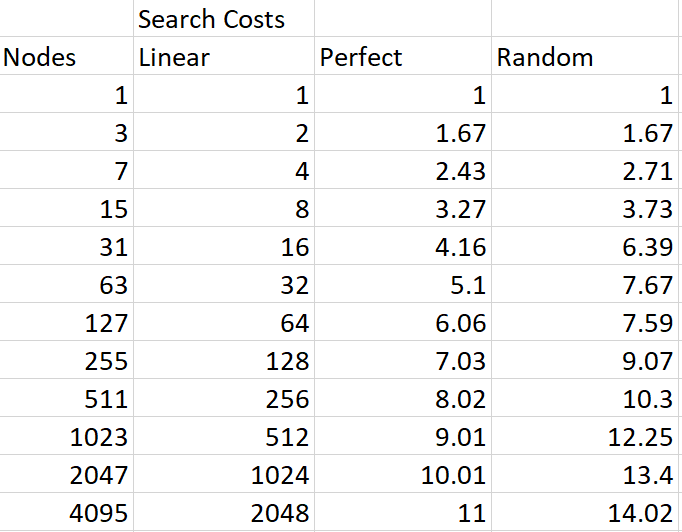
\includegraphics[width=7cm,height=\textheight,keepaspectratio]{BSTreeData.png} |
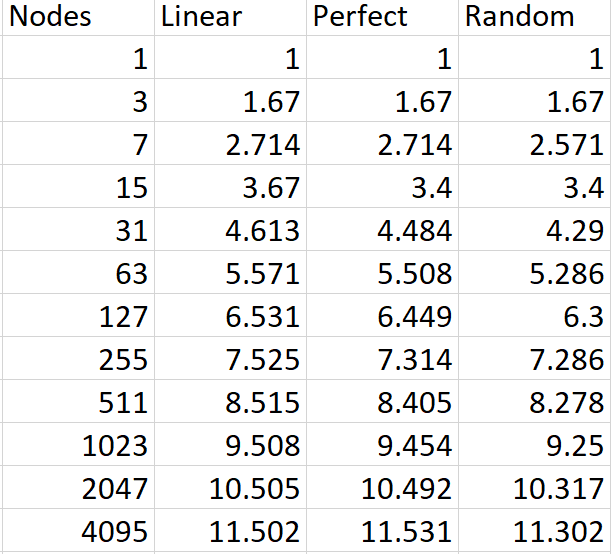
\includegraphics[width=\textwidth,height=5cm,keepaspectratio]{RBTreeData.png}\ \\




\ \\ \\ 
\ \\ \\ \\ \ \\\
\ \ \ \ \ \ \ \ \ \ \ \ \ \ \ \ \textbf{BinarySearchTree} \ \ \ \ \ \ \ \ \ \ \ \ \ \ \ \ \ \ \ \ \ \ \ \ \ \ \ \ \ \ \ \ \ \ \ \ \ \ \ \ \textbf{RedBlackTree}\ \\


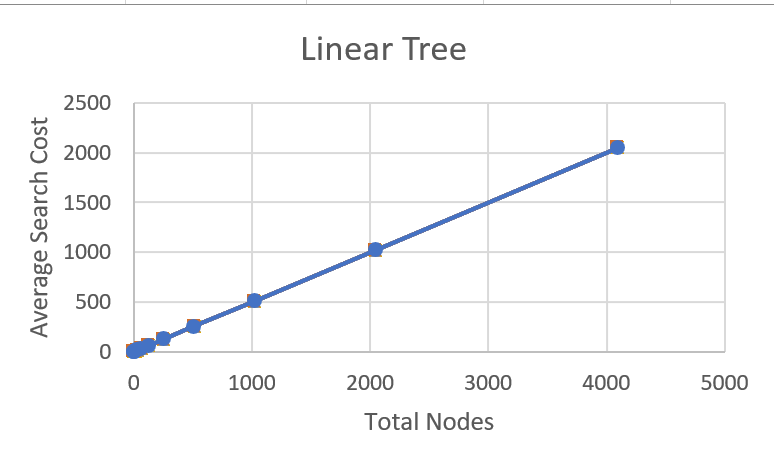
\includegraphics[width=7cm,height=\textheight,keepaspectratio]{BSTreeLinearPlot.png}
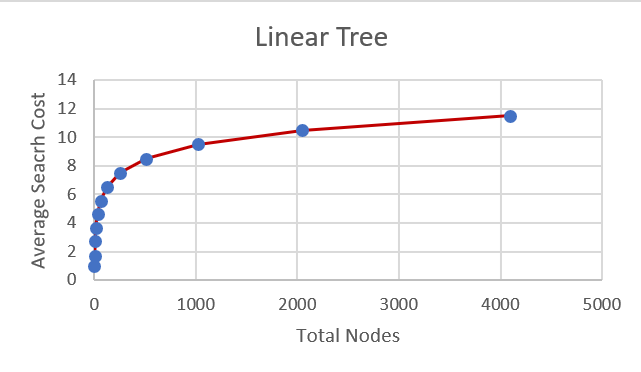
\includegraphics[width=7cm,height=\textheight,keepaspectratio]{RBTreeLinearPlot.png}\ \\
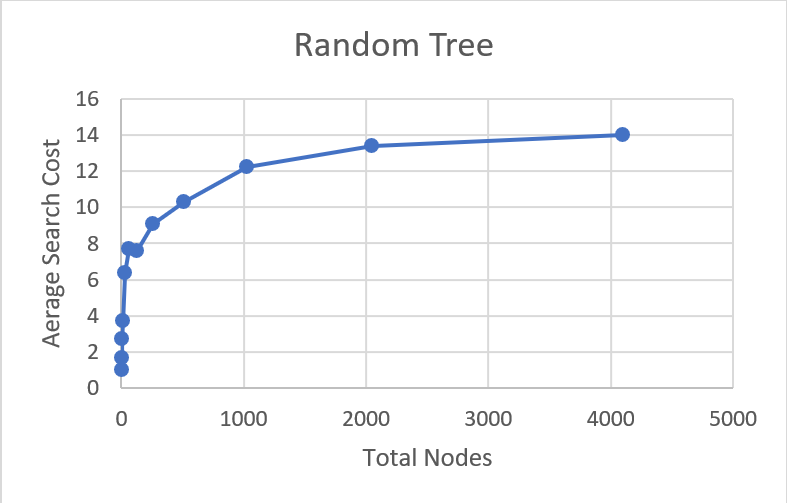
\includegraphics[width=7cm,height=\textheight,keepaspectratio]{BSTreeRandomPlot.png}
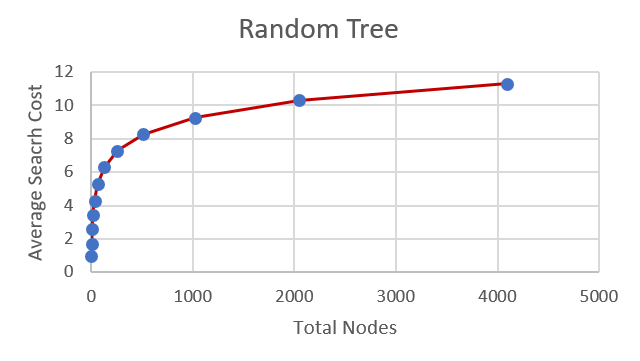
\includegraphics[width=7cm,height=\textheight,keepaspectratio]{RBTreeRandomPlot.png}\ \\
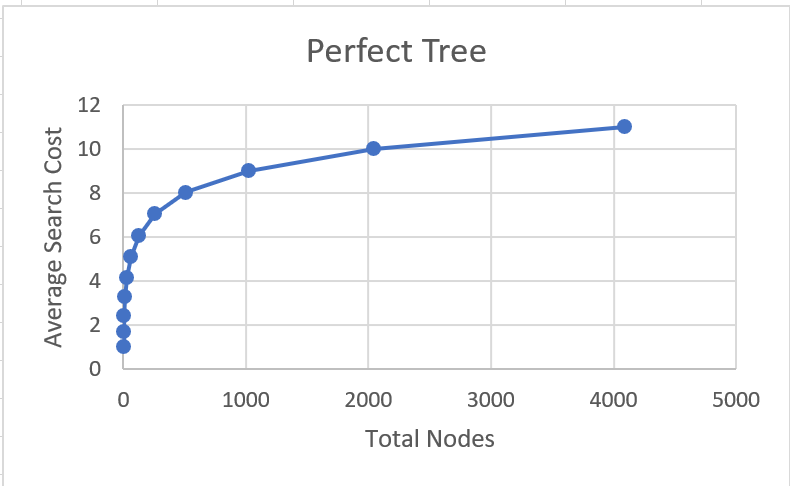
\includegraphics[width=7cm,height=\textheight,keepaspectratio]{BSTreePerfectPlot.png}
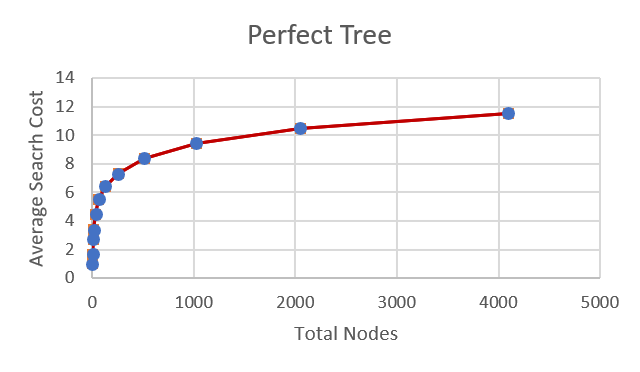
\includegraphics[width=7cm,height=\textheight,keepaspectratio]{RBTreePerfectPlot.png}\ \\
\ \\
Theoretical Upper and Lower Bounds\ \\
\textbf{Red-Black Tree} \ Upper: O(logn) Lower: O(logn) (Amortized)\ \\
\textbf{Binar Seacrh Tree} \ Upper: O(n) Lower: O(logn)\ \\
\ \\
\textit{Conclusion}\ \\
\ \\
Red-black trees greatly improve the search time for data that is unsorted. The benefit of using this method over a normal binary search tree increases as the data becomes more unsorted. Inversely, data that has previously been sorted will not benefit as greatly or at all from a red-black tree. The results show that perfect sorted data search times are actually negatively impacted by red-black trees.

\ \\
\item Include the testing cases for the small input data (the number of
nodes less than 16) for the files selected by you in the report.\ \\
\ \\
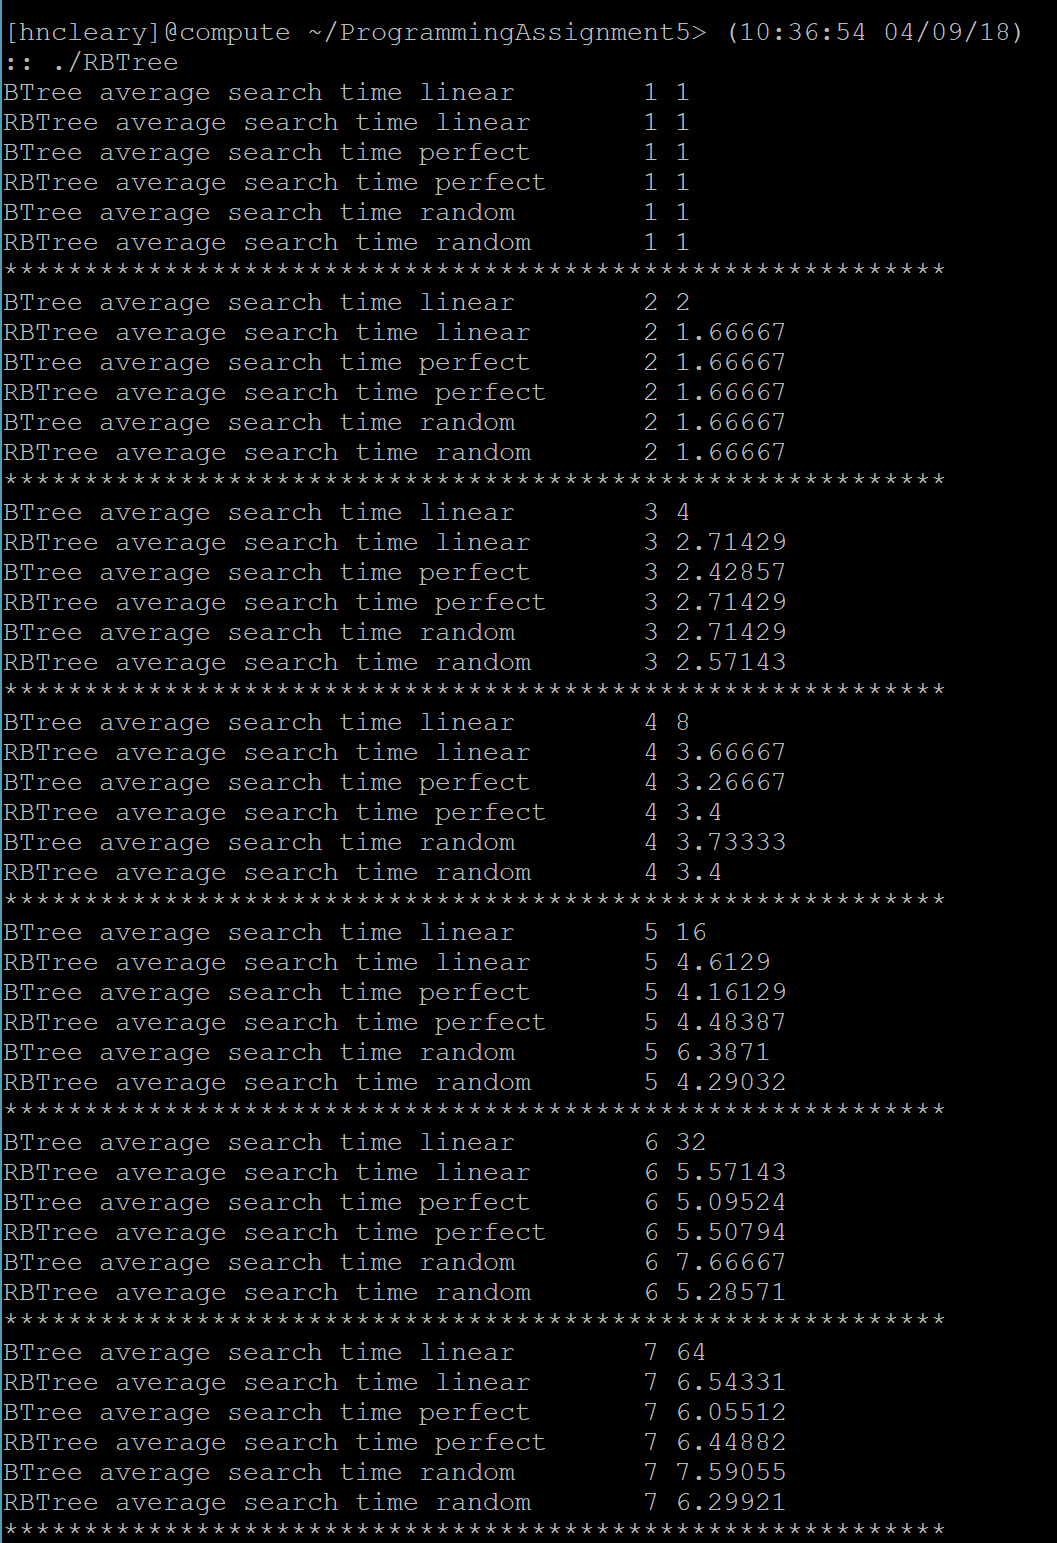
\includegraphics[width=9cm,height=\textheight,keepaspectratio]{putty_RBTree_Output.png}\ \\
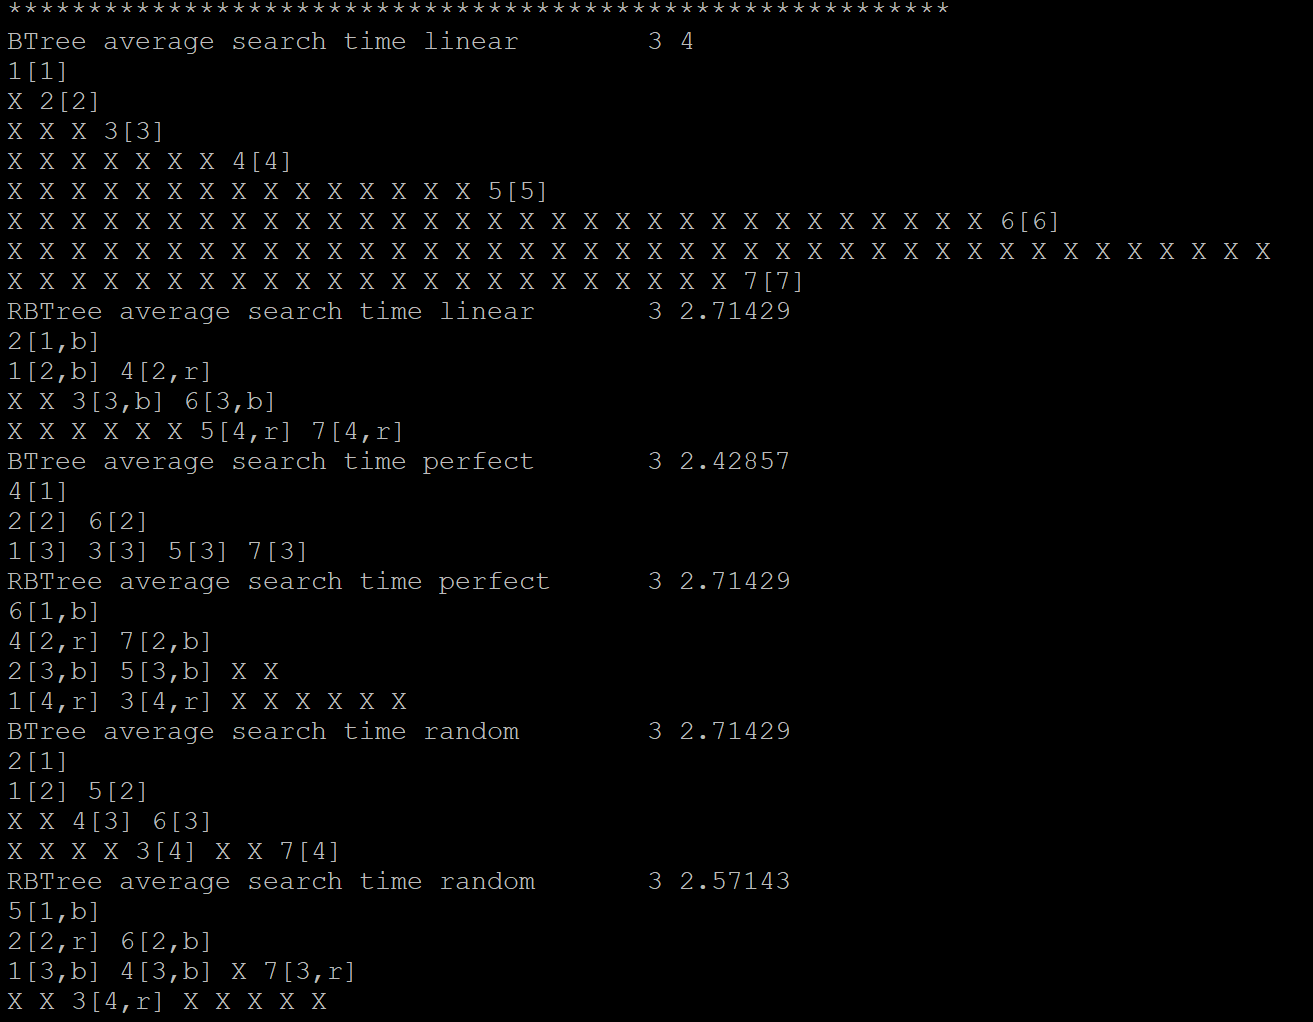
\includegraphics[width=9cm,height=\textheight,keepaspectratio]{puttyScreen.png}\ \\
\ \\
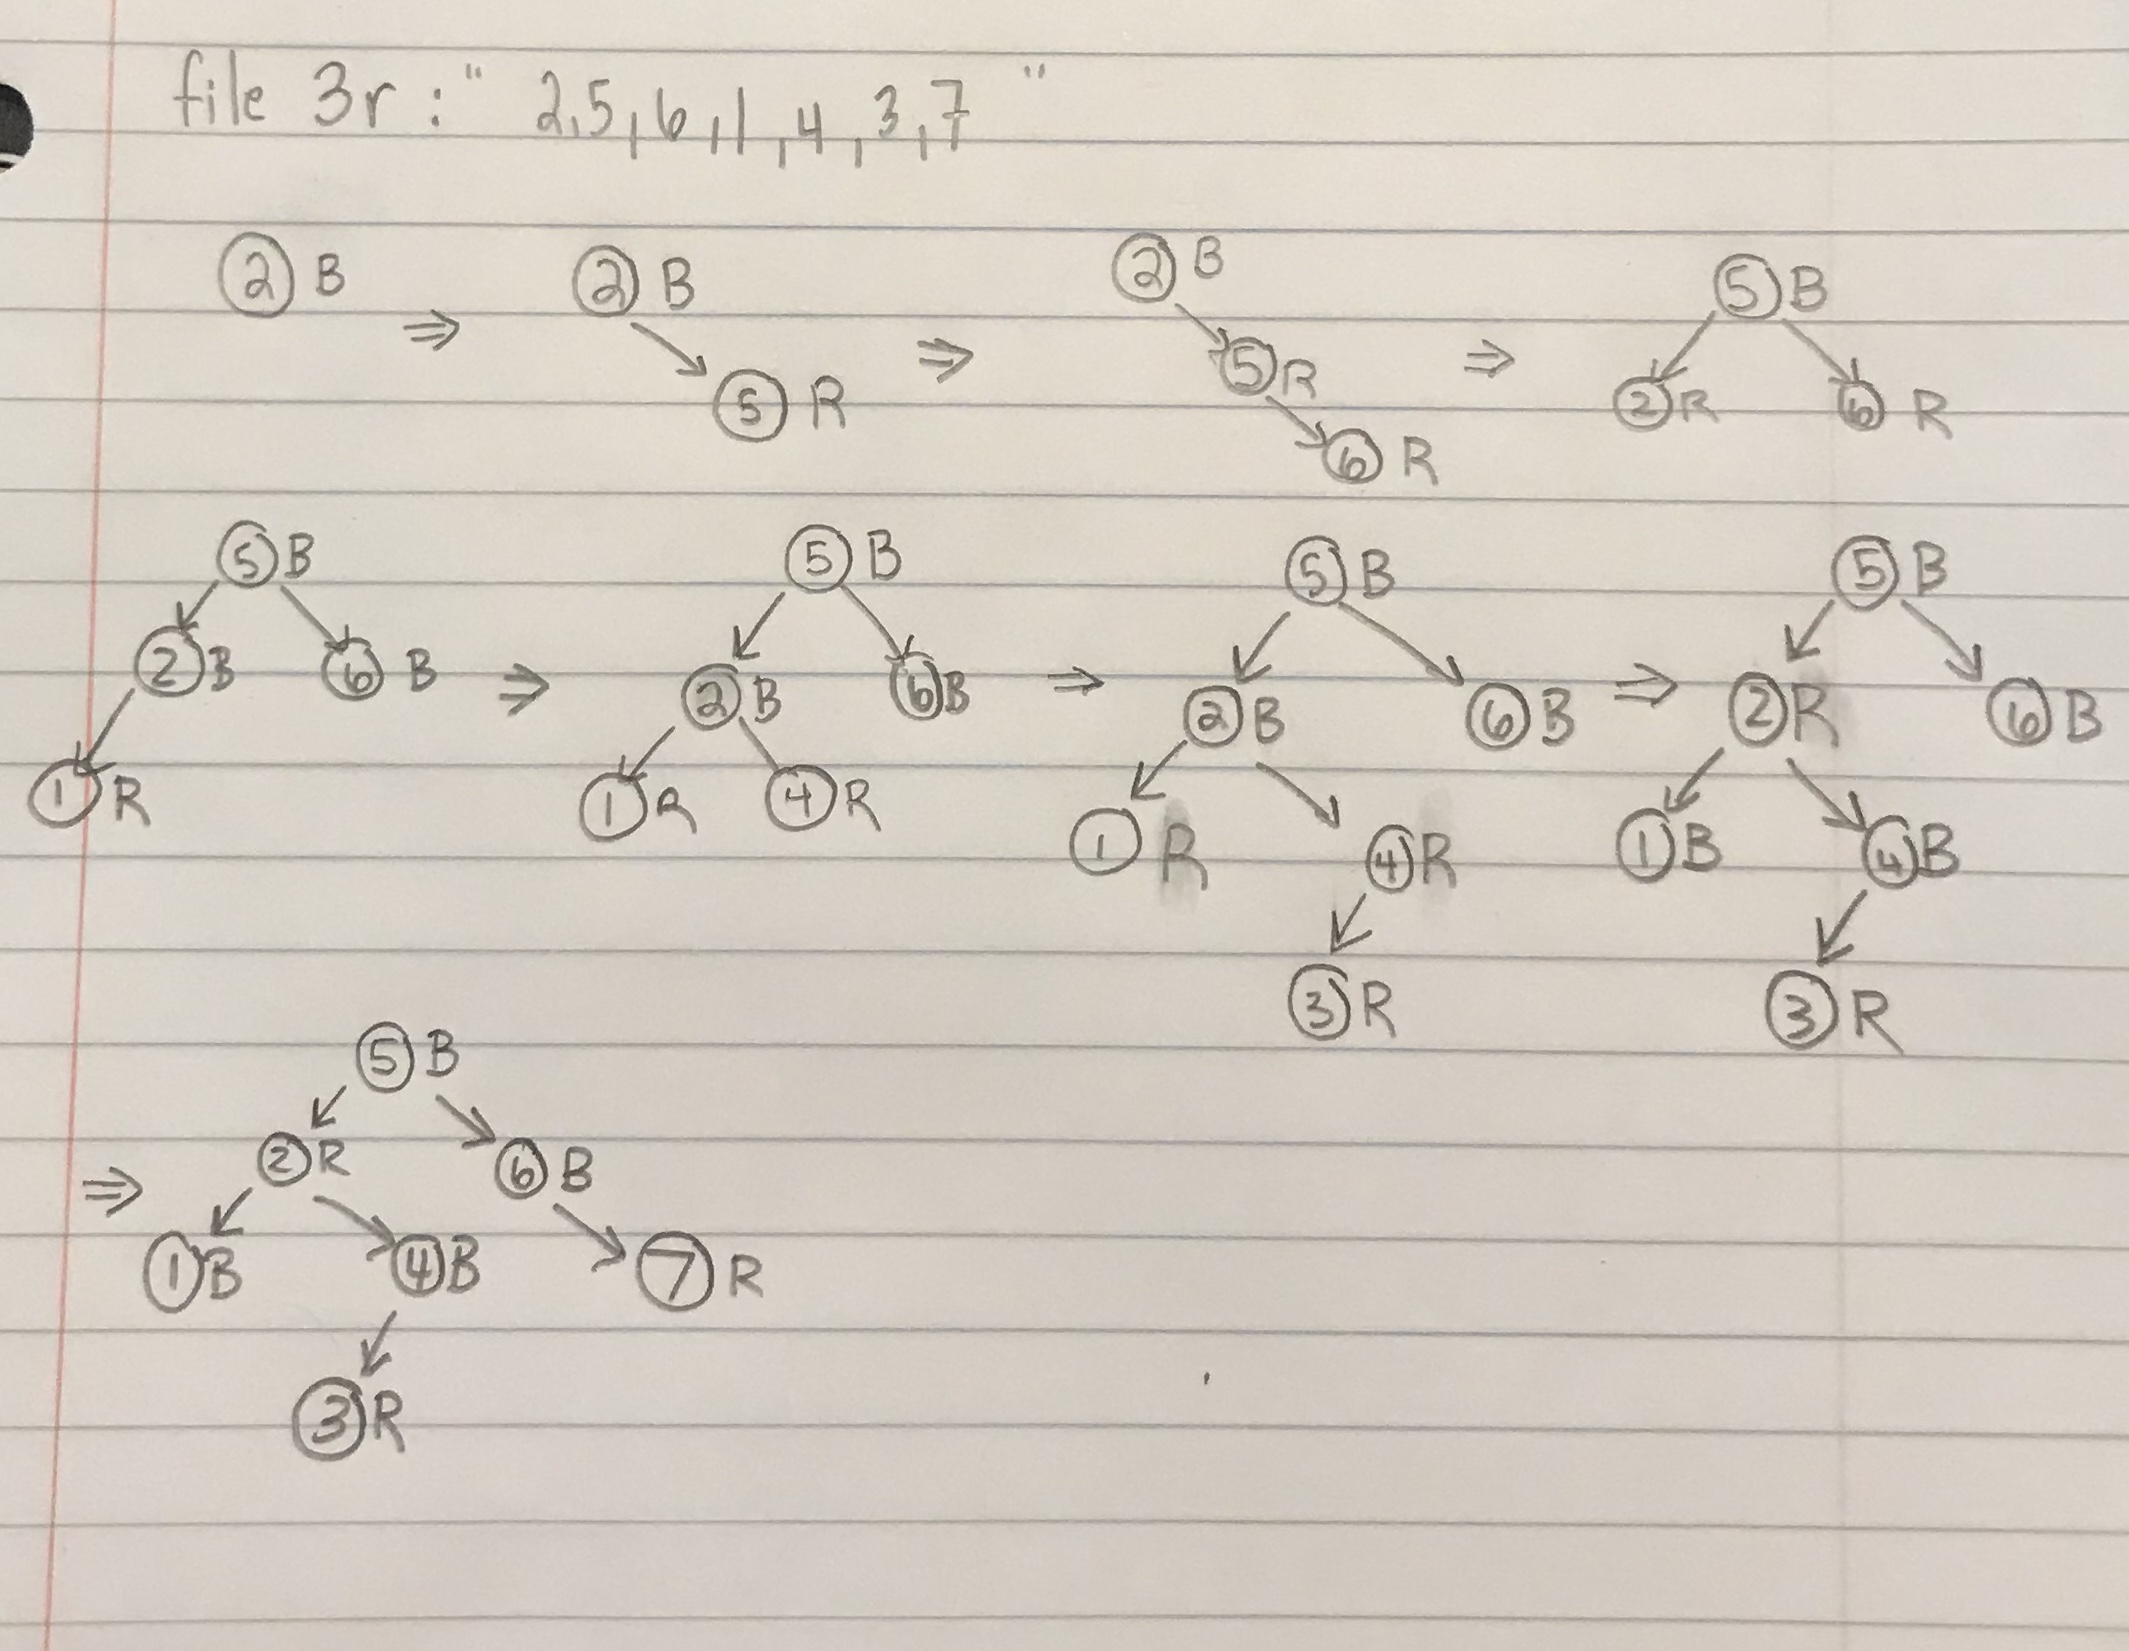
\includegraphics[width=9cm,height=\textheight,keepaspectratio]{IMG_3122.jpg}\ \\




\ \\
\item Summary. What have you learned by doing the assignment?\ \\
\ \\
Red-black trees are a type of binary search that are self sorted. This guarantees a guaranteed search time of amortized O(logn). The added cost of sorting data upon creation of the tree greatly decreases the search costs of data later on, but if the data has been previously sorted it will negatively impact performance (in a small factor).  

\ \\
\end{enumerate}

\end{document}
